% =============== IHM ===============
\chapter{IHM}


% ------------- Interface de l'écran d'accueil ------------
\section{Interface de l'écran d'accueil}
\TODO{Anthony}

% description, comment fonctionne l'écran d'accueil et comment on interagit avec…

% ------------- Gestion des parties ------------
\subsection{Gestion des parties}
\TODO{Anthony}

% comment on peut faire pour jouer à une partie, création ou rejoindre…

% ------------- Interface d'une partie en cours ------------
\section{Interface d'une partie en cours}
%\TODO{Simon}
% description de l'interface, pourquoi…
La figure~\ref{fig:ecran_partie} montre les fonctionnalités de l'application au cours d'une partie. On peut voir sur cette figure trois parties :
\begin{itemize}
	\item l'écran de jeu : c'est dans cette partie qu'est affiché le labyrinthe, on peut suivre sur cet écran les déplacements des joueurs, chaque joueur étant représenté par une couleur ;
	\item la liste des joueurs : cette partie montre la liste des joueurs et la couleur associé à chacun des joueurs, le joueur dont c'est le tour est également mis en évidence dans cette partie ;
	\item la console d'information : les informations, qui décrivent le dernier tour joué, s'affichent dans cette console, la console affiche donc un descriptif de tous les tours joués jusqu'à lors.
\end{itemize}
\begin{figure}[h]
	\centering
	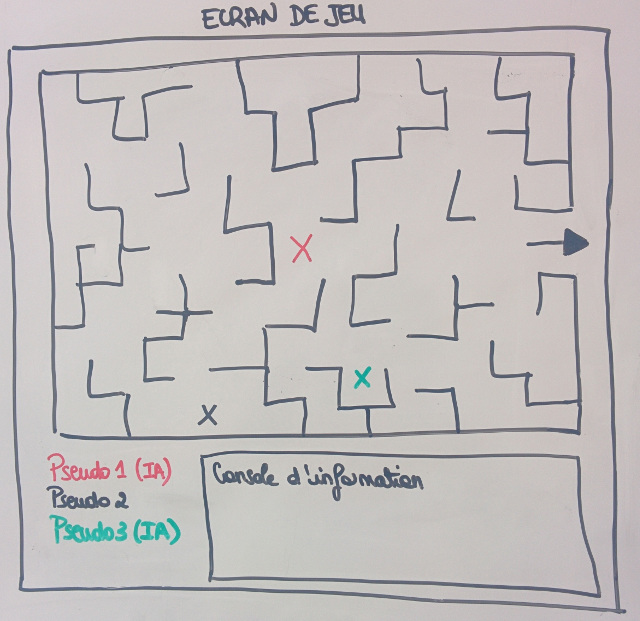
\includegraphics[scale=0.2]{images/schema_ecran_partie.jpg}
	\caption{Schéma de l'écran d'une partie}
	\label{fig:ecran_partie}
\end{figure}

% ------------- Gestion des déplacements ------------
\subsection{Gestion des déplacements}
%\TODO{Simon}
% comment sont gérer les déplacements humains ou bot
À chaque tour, un joueur dispose d'un temps limité pour indiquer son déplacement. Ce déplacement peut être : "HAUT", "BAS", "GAUCHE", "DROITE". À la fin du tour, le déplacement est effectué. On distingue deux manières de jouer : avec une IA ou sans IA.
\subsubsection*{Déplacement humain}
Lorsqu'un joueur joue sans IA, il dispose d'un temps supérieur pour indiquer son déplacement. Il indique son déplacement à l'aide des touches fléchées. Dans le cas où le joueur ne veut pas se déplacer, il peut appuyer sur la touche espace pour passer son tour. Dans le cas où il n'appuie sur aucune touche avant la fin du temps imparti, il ne se déplace pas. Dans le cas où son déplacement n'est pas valide, par exemple si la destination est un mur, il ne se déplace pas non plus.
\subsubsection*{Déplacement avec une IA}
À chaque tour, l'IA dispose d'un temps pour indiquer son déplacement. Le programme indique son déplacement sous la forme d'une chaîne de caractère ("HAUT", "BAS", "GAUCHE" ou "DROITE"). Si la chaine de caractère est mal formée, où si le programme met trop de temps à répondre, le joueur ne se déplace pas. De la même manière que pour les joueurs humains, si le déplacement n'est pas valide, il n'est pas pris en compte.